% !TeX root = ../../../main.tex
\subsection{Full Experimental Results}\ChThreeHeadingOnly
\label{ch03:apd:full_results}




\subsubsection{Survival Analysis Model Performance across 9 and 12 months Snapshots}
\label{ch03:apd:survival_analysis}

The prediction performance of the survival analysis models across 9 and 12 months snapshots is summarized in Table~\ref{ch03:tab:survival_9_12}.
Similar to earlier time points presented in Table~\ref{ch03:tab:survival_3_6}, the Random Survival Forest consistently outperforms other models in terms of discriminative ability and calibration.
At 9 months, it achieves the highest Concordance Index (\(C^{td} = 0.648 \pm 0.015\)) and time-dependent AUC (\(\text{AUC}^{td} = 0.694 \pm 0.015\)), along with the lowest Integrated Brier Score (\(\text{IBS} = 0.180 \pm 0.003\)).
At 12 months, the Random Survival Forest maintains its superior performance with \(C^{td} = 0.658 \pm 0.011\), \(\text{AUC}^{td} = 0.706 \pm 0.011\), and \(\text{IBS} = 0.174 \pm 0.004\).

CoxPH and DeepSurv display competitive performance at 9 months, with CoxPH maintaining slightly higher \(C^{td}\) scores (\(0.625 \pm 0.023\)) and comparable calibration as indicated by its \(\text{IBS} = 0.187 \pm 0.004\).
DeepSurv exhibits strong calibration at 9 months (\(\text{IBS} = 0.185 \pm 0.004\)), though it trails behind Random Survival Forest in overall predictive metrics.
By 12 months, DeepSurv demonstrates modest gains, but CoxPH results are unavailable for this time point.

DeepHit continues to underperform across these later snapshots, with \(C^{td}\) values of \(0.525 \pm 0.069\) at 9 months and \(0.540 \pm 0.026\) at 12 months, indicating weaker discriminative ability.
Similarly, its higher \(\text{IBS}\) values (\(0.234 \pm 0.026\) at 9 months and \(0.243 \pm 0.021\) at 12 months) suggest poorer calibration.
These trends highlight DeepHit's limitations in handling the low-dimensional and moderate-sized dataset used in this study.
Given these limitations, the use of DeepHit in our causal inference meta-learner approach for predicting restricted mean time (RMET) is unreliable, as its survival estimates lack the necessary stability and accuracy.


% !TeX root = ../../../main.tex
\begin{table}[!htbp]
    \setlength{\tabcolsep}{2pt}
    \ChThreeFloatContents
      {ch03:tab:survival_9_12}
      {\caption{Prediction Performance Across Time Snapshots (9 and 12 months)}}
      {\adjustbox{max width=.9\textwidth}{\begin{tabular}{l  c c c @{\hspace{0.5cm}} c c c }
    \toprule
    \textbf{Snapshot Time}&\multicolumn{3}{c}{9 months} & \multicolumn{3}{c}{12 months} \\
    \midrule
     & \(C^{td}\) & IBS & \(\text{AUC}^{td}\) & \(C^{td}\) & IBS & \(\text{AUC}^{td}\) \\
    \midrule
    CoxPH & 0.625 ± 0.023 & 0.187 ± 0.004 & 0.664 ± 0.025 & 0.630 ± 0.024 & 0.195 ± 0.010 & 0.672 ± 0.023 \\
    Random Survival Forest & {\ChThreeBfTab 0.648} ± 0.015 & {\ChThreeBfTab 0.180} ± 0.003 & {\ChThreeBfTab 0.694} ± 0.015 & {\ChThreeBfTab 0.658} ± 0.011 & {\ChThreeBfTab 0.174} ± 0.004 & {\ChThreeBfTab 0.706} ± 0.011 \\
    DeepSurv & 0.630 ± 0.009 & 0.185 ± 0.004 & 0.668 ± 0.011 & 0.636 ± 0.013 & 0.187 ± 0.010 & 0.675 ± 0.016 \\
    DeepHit & 0.525 ± 0.069 & 0.234 ± 0.026 & 0.556 ± 0.065 & 0.540 ± 0.026 & 0.243 ± 0.021 & 0.558 ± 0.014 \\
    \bottomrule
    \end{tabular}}}
\end{table}


Overall, the results reinforce the performance advantage of the Random Survival Forest across varying time horizons, making it the most reliable model evaluated for predicting time-to-first-event in our dataset.
However, even with \(C^{td}\) values consistently above 0.6, there remains significant room for improvement in survival modeling.
This gap in predictive accuracy introduces a caveat for our causal inference analyses, as the reliability of causal estimates is contingent on the underlying survival model's performance.
Addressing this limitation is critical for advancing both predictive and causal modeling in similar clinical contexts.

\subsubsection{Full Causal Inference Results across 9 and 12 months Snapshots}
\label{ch03:apd:causal_inference}


% !TeX root = ../../../main.tex
\begin{table}[!hbtp]
    \setlength{\tabcolsep}{4pt}
    \ChThreeFloatContents
      {ch03:tab:table_ate_9_12}
      {\caption{Causal Inference ATE Estimates at 9 and 12 Months}}
      {\adjustbox{max width=.825\textwidth}{\begin{tabular}{l c c c c c }
    \toprule
    &T-learner & S-learner & Matching (1) & Matching (5) & Matching (20) \\
    \midrule
    \textit{(Snapshot: 9 months)} \\
    CoxPH & -2.285 ± 0.578 & -1.384 ± 0.512 & -1.658 ± 0.006 & -1.790 ± 0.002 & -2.032 ± 0.003 \\
    Random Survival Forest & -1.468 ± 0.518 & -0.546 ± 0.106 & -1.159 ± 0.042 & -1.242 ± 0.050 & -1.540 ± 0.055 \\
    DeepSurv & -2.144 ± 2.706 & 0.837 ± 0.767 & -0.923 ± 0.446 & -0.928 ± 0.436 & -1.021 ± 0.558 \\
    DeepHit & 6.887 ± 5.930 & 0.169 ± 0.692 & -0.160 ± 0.344 & -0.168 ± 0.328 & -0.163 ± 0.368 \\
    \midrule
    Causal Survival Forest &  \multicolumn{5}{c}{-1.610 ± 0.057 (Not a meta-learner method)}  \\
    \midrule \\
    \textit{(Snapshot: 12 months)} \\
    Random Survival Forest & 0.099 ± 0.430 & 0.050 ± 0.173 & -0.427 ± 0.148 & -0.544 ± 0.134 & -0.829 ± 0.127 \\
    DeepSurv & -2.650 ± 1.553 & 1.116 ± 0.605 & 0.262 ± 1.353 & -0.025 ± 1.381 & -0.347 ± 1.399 \\
    DeepHit & 0.822 ± 3.215 & 1.021 ± 0.535 & 0.355 ± 0.424 & 0.256 ± 0.420 & 0.148 ± 0.415 \\
    \midrule
    Causal Survival Forest &  \multicolumn{5}{c}{0.345 ± 0.097 (Not a meta-learner method)}  \\
    \bottomrule
    \end{tabular}}}
\end{table}


The Average Treatment Effect (ATE) estimates for 9 and 12 months are summarized in Table~\ref{ch03:tab:table_ate_9_12}.
At 9 months, we observe predominantly negative ATEs across most models, suggesting that non-adherence is associated with shorter adverse event times to adverse events, consistent with expectations.
However, by 12 months, there is a notable increase in positive ATE estimates, indicating that adherence might correspond to shorter adverse event times to adverse events, which contradicts clinical expectations.

Examining the standard errors of the ATE estimates across different experimental repeats provides additional context for the unreliability of these numbers for longer time snapshots.
For example, while some negative ATEs at 9 months align with expectations, large standard errors, such as those seen for DeepSurv (\(-2.144 \pm 2.706\)), reduce confidence in these estimates.
Similarly, small ATE magnitudes close to zero, such as those reported by Random Survival Forest using the S-learner (\(-0.546 \pm 0.106\)), suggest minimal difference between adherence and non-adherence.

This unexpected trend of positive ATEs at 12 months can be attributed to two primary factors.
First, the underlying survival models at these later snapshots demonstrate weaker performance compared to earlier snapshots, as discussed in Appendix~\ref{ch03:apd:survival_analysis}.
This degradation in survival model accuracy likely propagates to the causal inference estimates, introducing additional unreliability.
Second, there is an inherent bias in the sampled cohort for these later snapshots.
By definition, for each time snapshot, its corresponding cohort consists of individuals who have not experienced an adverse event up to the later time points, regardless of their previous adherence history.
This selection process results in a subgroup that may not be representative of the full cohort, as it comprises patients with inherently better survival probabilities.
Specifically, individuals who survive to later time points without experiencing an adverse event are likely to have more favorable unmeasured health characteristics or environmental factors that contribute to their prolonged survival.
This could include better baseline health, fewer comorbid conditions, or access to additional social or medical resources not captured in the data.
As a result, the sampled cohort at these later time points is disproportionately composed of patients who are less likely to experience adverse events, irrespective of their adherence behavior.
Consequently, the observed ATE estimates at later snapshots are influenced by this selection bias, further complicating their interpretation.

From these results, we observe that the performance and reliability of causal inference analyses at later time points are diminished.
For instance, at 12 months, Random Survival Forest reports ATEs close to zero (\(0.099 \pm 0.430\) for the T-learner and \(0.050 \pm 0.173\) for the S-learner), indicating negligible differences between adherence and non-adherence.
Additionally, the large standard errors in estimates such as those from DeepSurv (\(1.116 \pm 0.605\)) and DeepHit (\(1.021 \pm 0.535\)) highlight the lack of reliability in these results.

The increased presence of positive ATEs highlights the compounded effects of weaker survival models and cohort selection bias.
While these findings provide some insights, they emphasize the need for cautious interpretation and underscore the importance of addressing these limitations in future analyses.

\subsubsection{Graphical Representation of ATE Trends Across Time Snapshots}
\label{ch03:apd:graphical_ate}

Figure~\ref{ch03:fig:graphical_ATE_trend} presents the Average Treatment Effect (ATE) estimates at different time snapshots \(\tau\) for the survival models experimented with (Cox Proportional Hazards (CoxPH), Random Survival Forest, DeepSurv, and DeepHit).
Each subfigure illustrates the ATE trends over time for a specific survival model, incorporating multiple meta-learning approaches.
To facilitate comparisons, the Causal Survival Forest (CSF) that is inherently a causal method is included in all plots.


% !TeX root = ../../../main.tex
\begin{figure}[!htp]
\ChThreeFloatContents
  {ch03:fig:graphical_ATE_trend}
  {\caption{Estimated Average Treatment Effect (ATE) of non-adherence across time snapshots \(\tau\) for different survival models. Each panel corresponds to a specific survival model (CoxPH, Random Survival Forest, DeepSurv, and DeepHit), with ATE estimates reported for multiple meta-learning approaches (T-learner, S-learner, and Matching). The Causal Survival Forest (CSF) is included in all plots as a baseline for comparison. Shaded regions represent standard deviations, illustrating the uncertainty in the estimates.}}
  {%
    \subfigure[CoxPH]{\label{ch03:fig:graphical_ate_coxph}%
      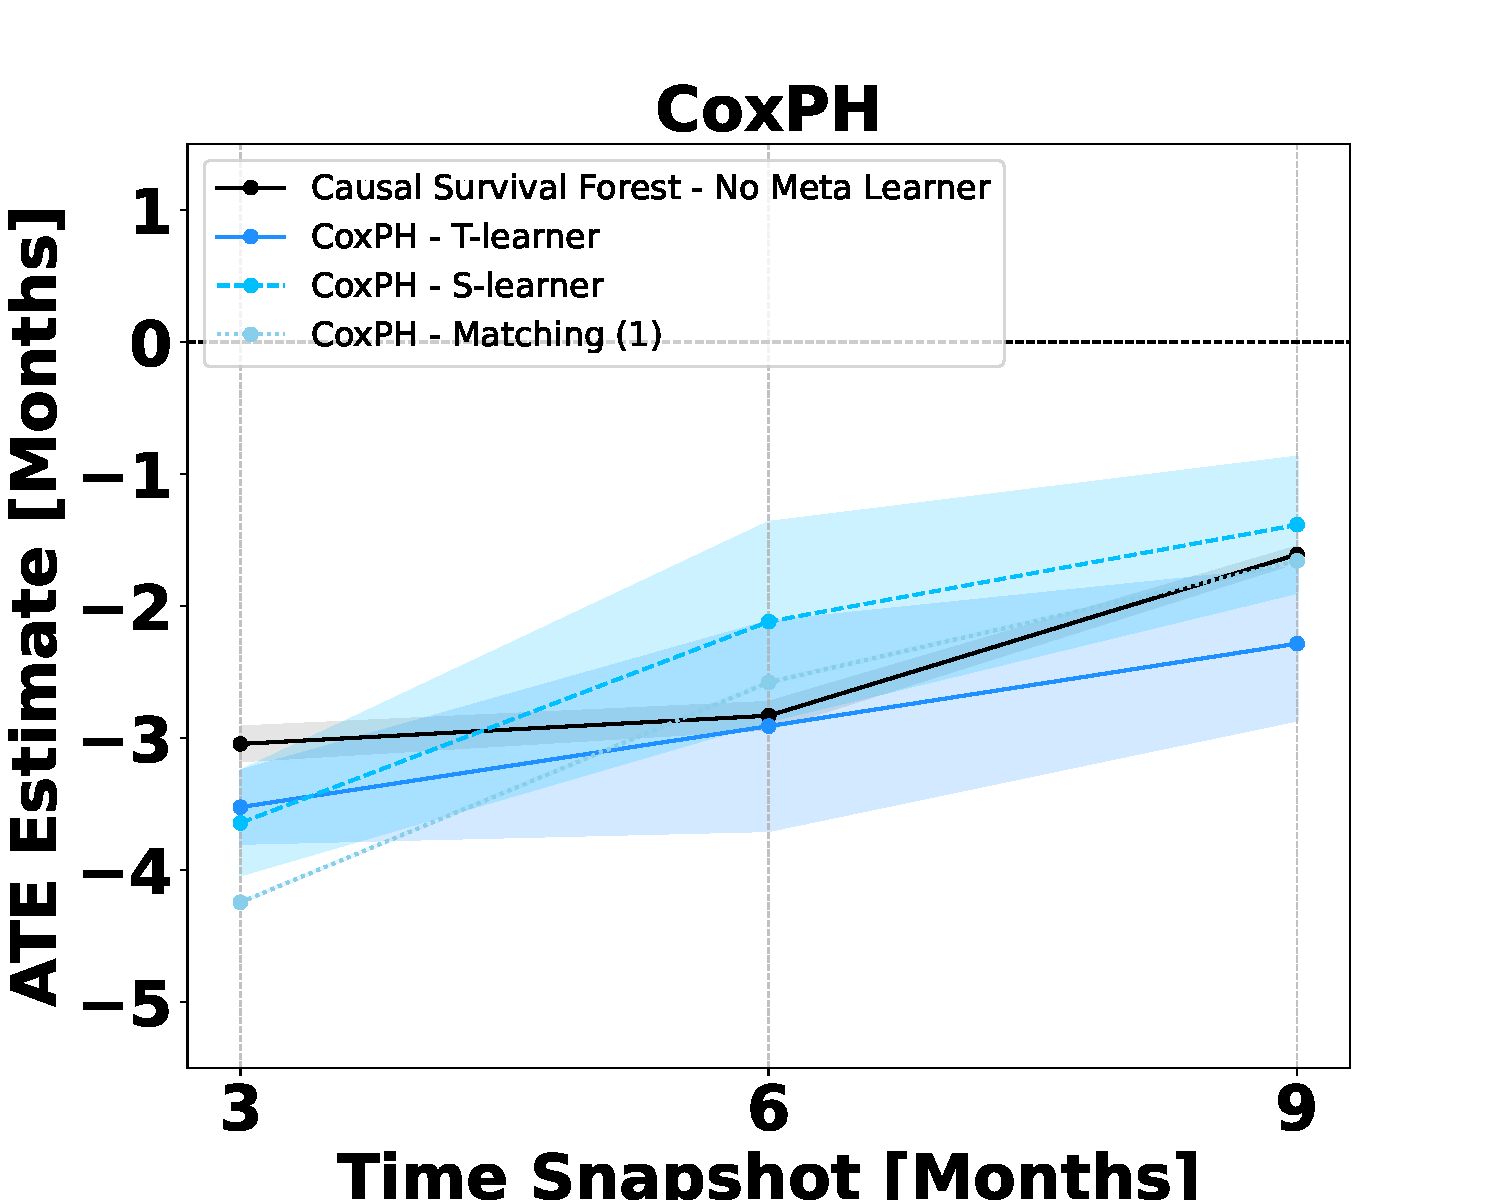
\includegraphics[width=.45\linewidth]{Appendices/appendix-ch03/images/Graphical_ATE/Graphical_ATE_CoxPH.pdf}}%
    \subfigure[RandomSurvivalForest]{\label{ch03:fig:graphical_ate_rsf}%
      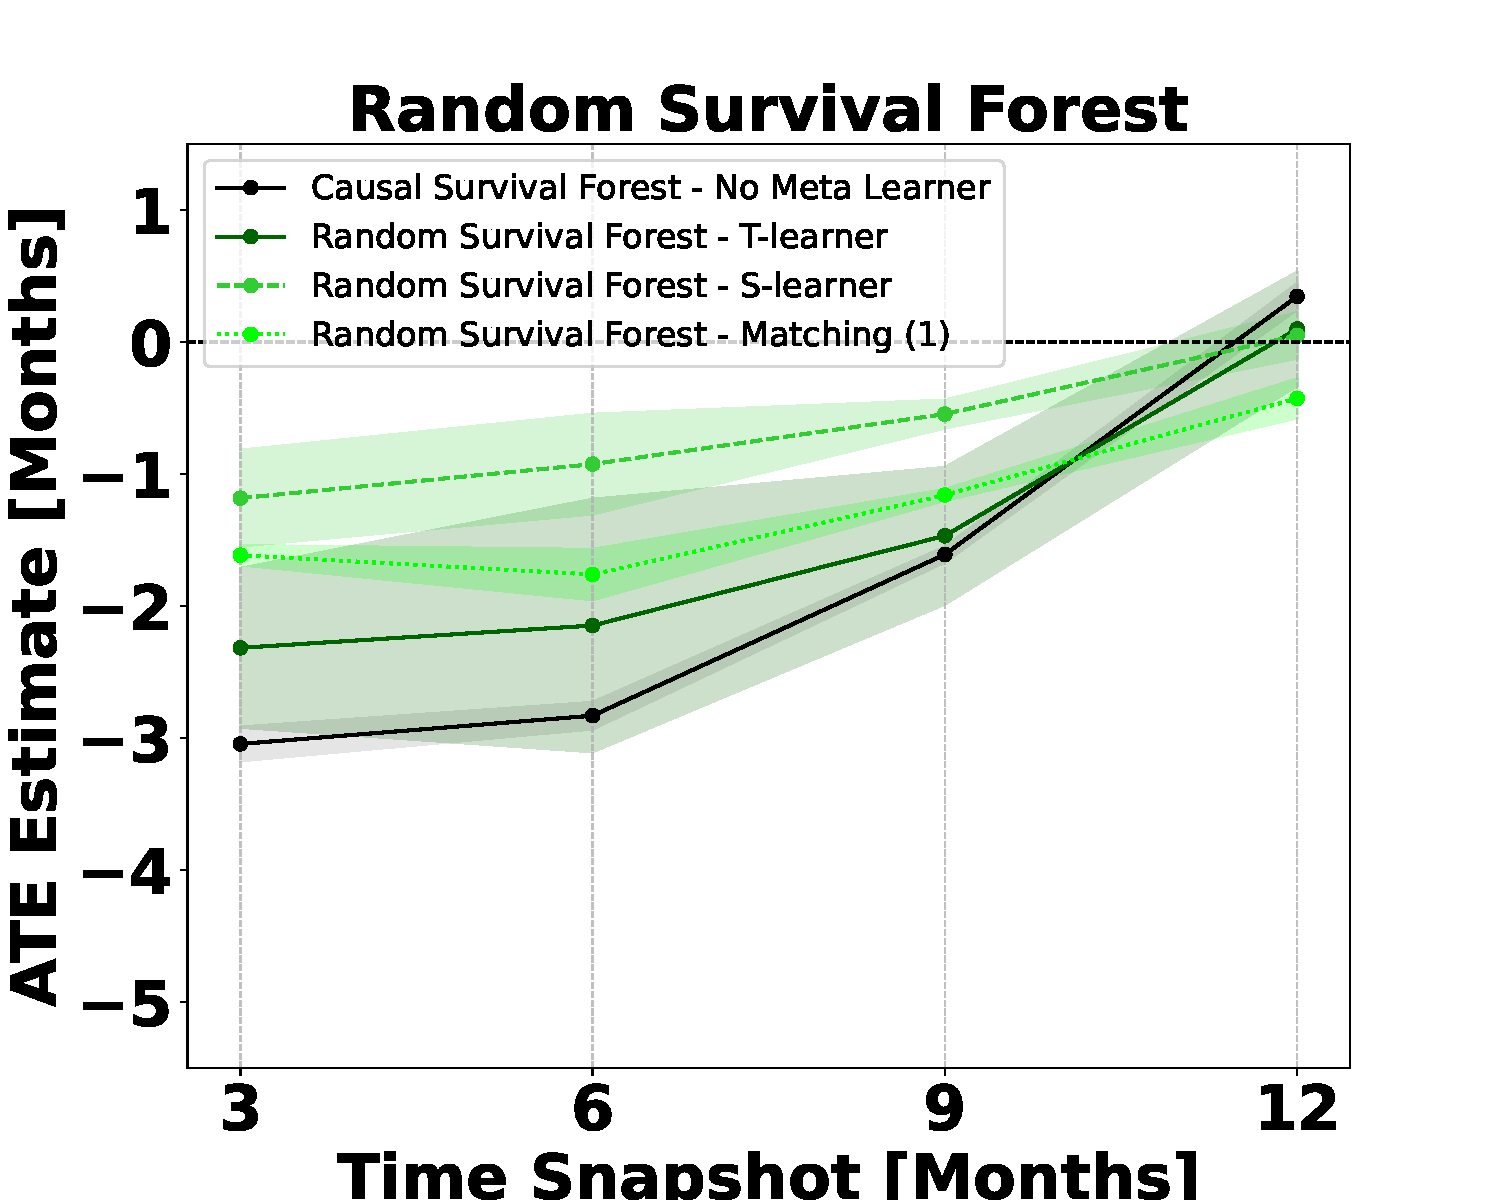
\includegraphics[width=.45\linewidth]{Appendices/appendix-ch03/images/Graphical_ATE/Graphical_ATE_Random_Survival_Forest.pdf}}%
      \\
    \subfigure[DeepSurv]{\label{ch03:fig:graphical_ate_deepsurv}%
      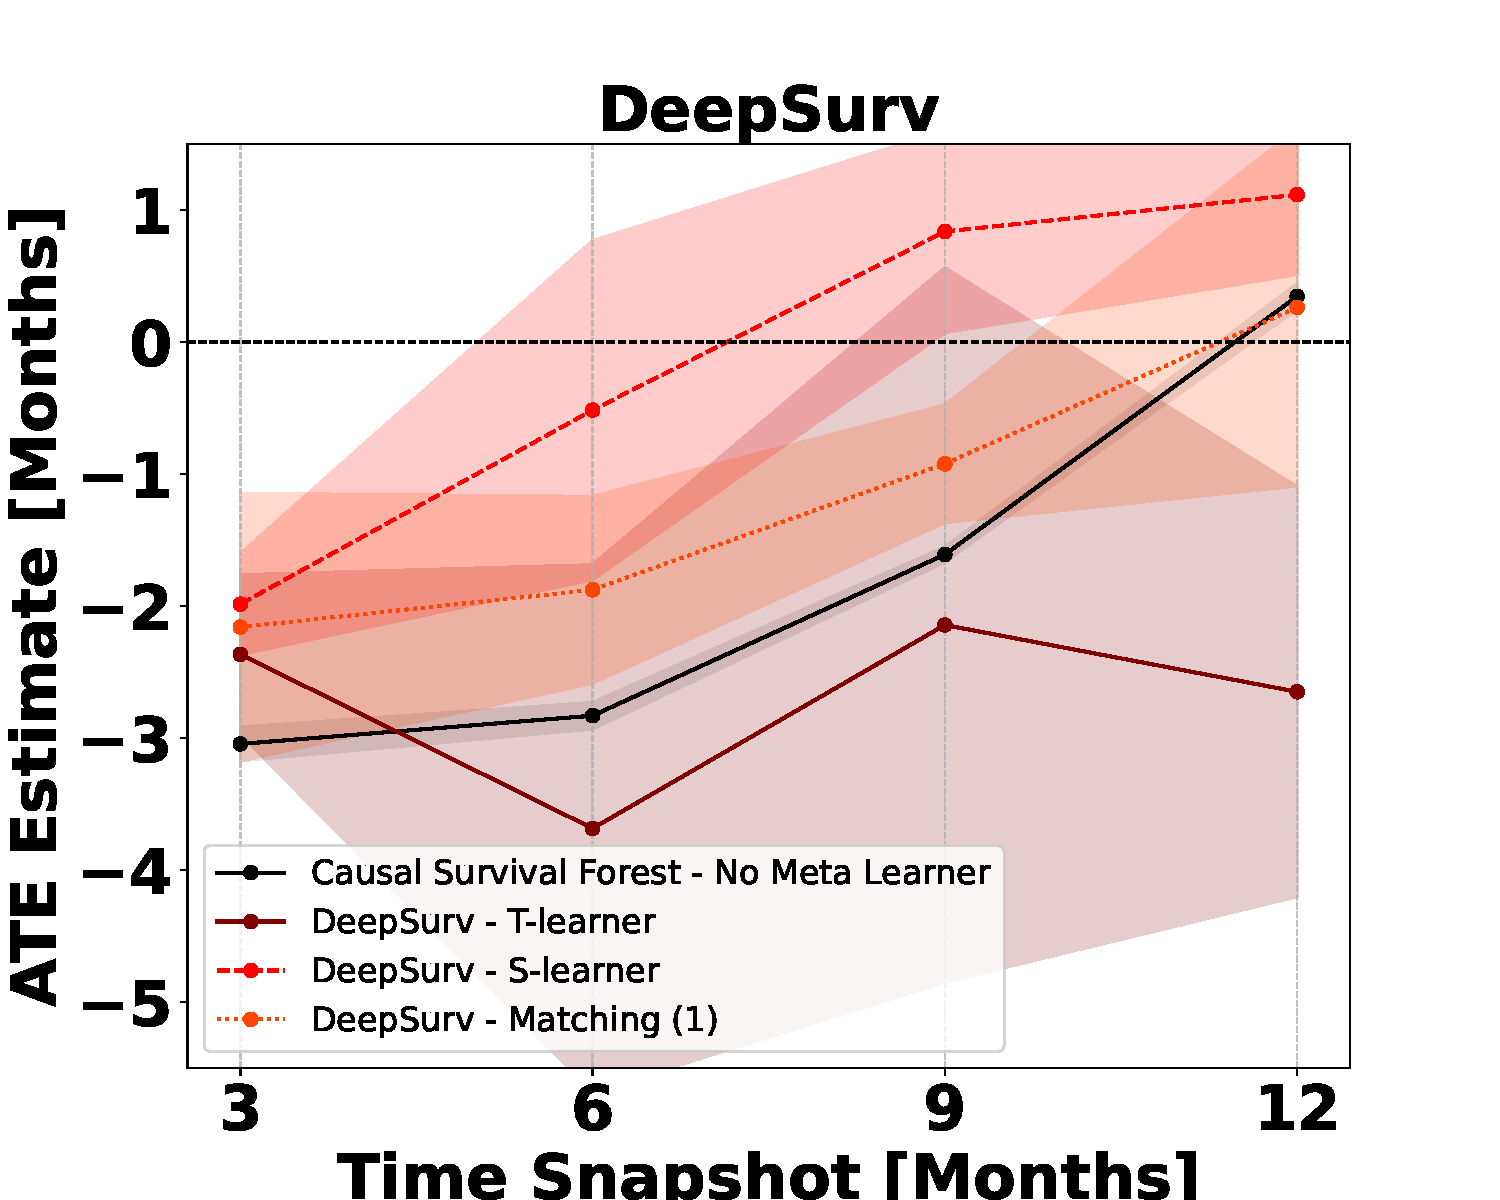
\includegraphics[width=.45\linewidth]{Appendices/appendix-ch03/images/Graphical_ATE/Graphical_ATE_DeepSurv.pdf}}%
    \subfigure[DeepHit]{\label{ch03:fig:graphical_ate_deephit}%
      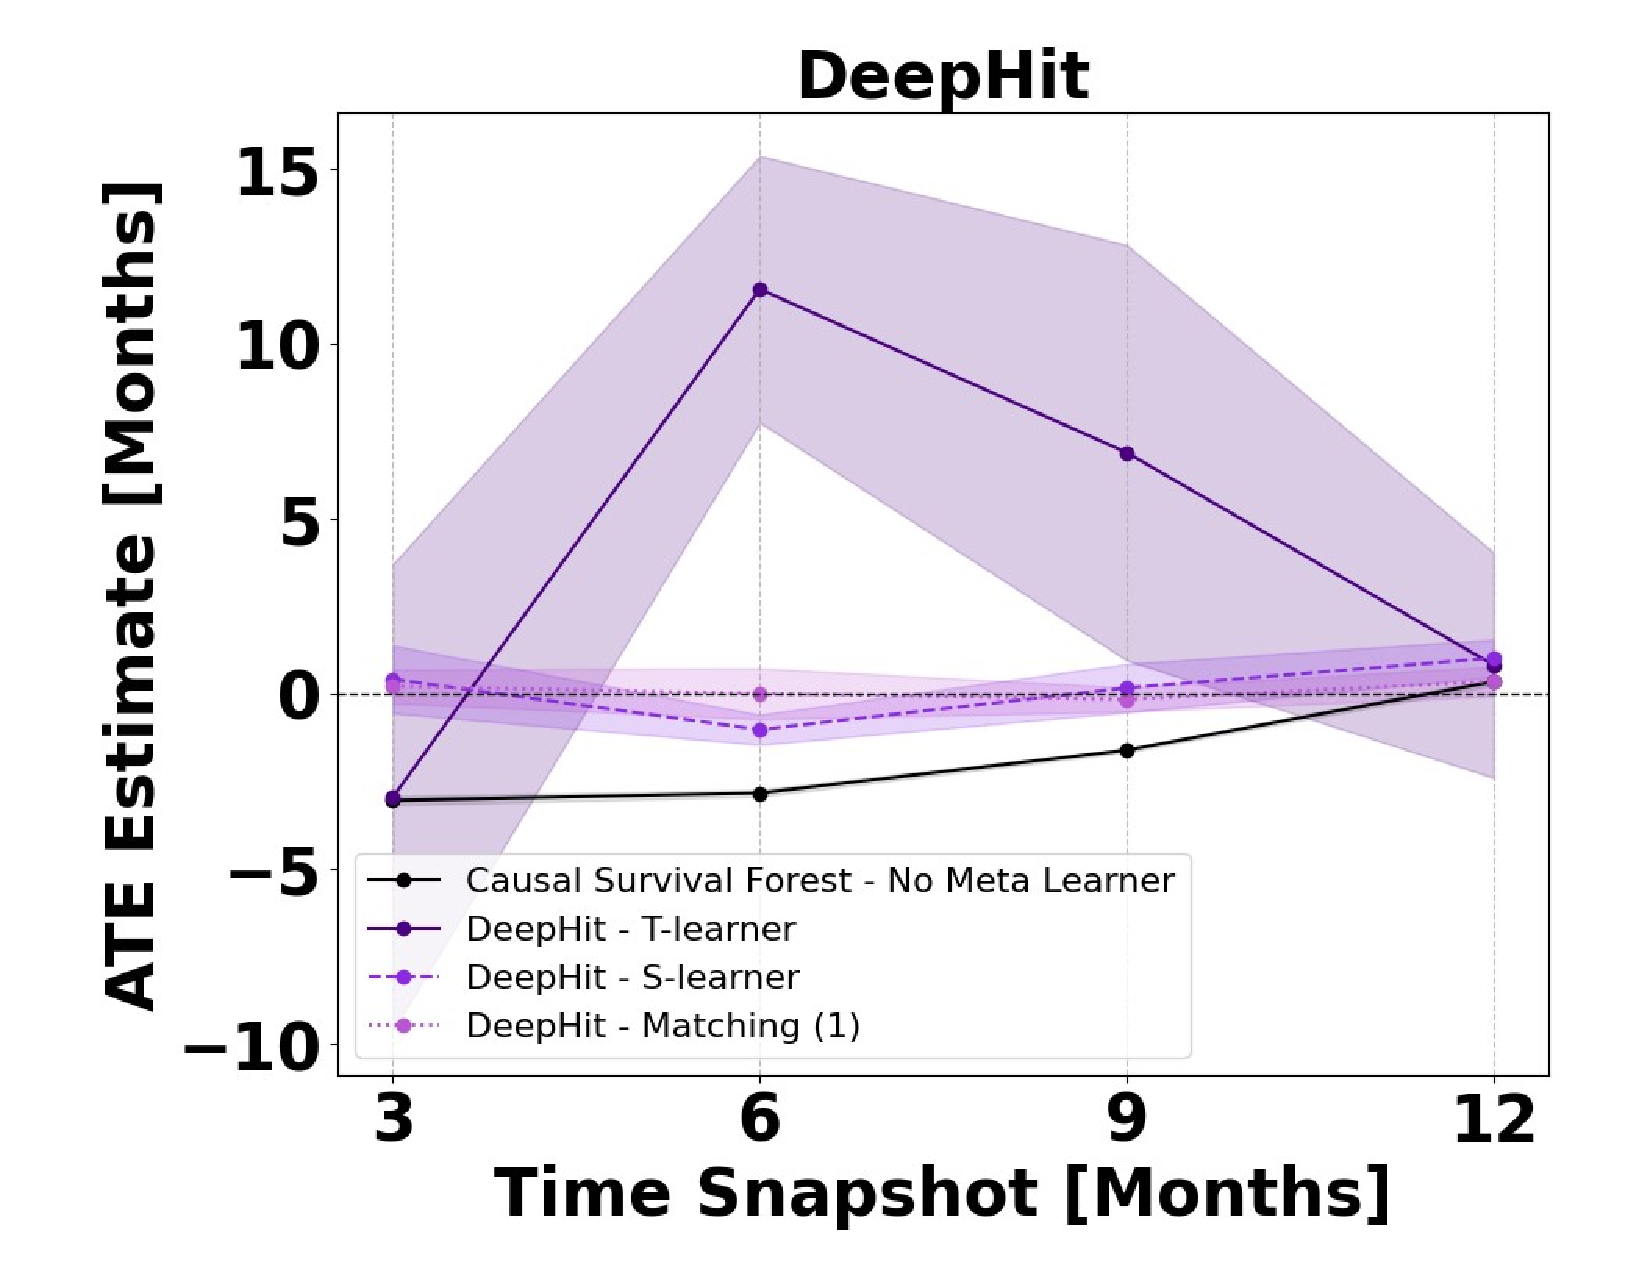
\includegraphics[width=.46\linewidth]{Appendices/appendix-ch03/images/Graphical_ATE/Graphical_ATE_DeepHit.pdf}}%
  }
\end{figure}


The graphical analysis of ATE estimates over time highlights consistent trends across different survival models and meta-learning strategies.
Across CoxPH, Random Survival Forest (RSF), and DeepSurv, a clear ranking of ATE estimates emerges, with the T-learner consistently producing the most negative values, the S-learner yielding the least negative values, and the Matching-based estimator falling in between.
This pattern holds across all time snapshots, suggesting that the T-learner amplifies the estimated effect of non-adherence, whereas the S-learner provides more conservative estimates.
The Causal Survival Forest (CSF), included in all plots, provides relatively stable estimates that align closely with those from RSF and CoxPH.

As time progresses, a general upward trend is observed in ATE estimates, with some models—particularly RSF and CSF—approaching zero or slightly positive values at 12 months.
However, this shift should be interpreted with caution, as it is likely influenced by \textit{survivor bias}, where the population at later time points consists only of individuals who have not yet experienced an adverse event.
As discussed in Section~\ref{ch03:sec:04_results_causal}, this selection dynamic skews the estimates toward a subset of individuals who may inherently be at lower risk, leading to a potential underestimation of the true treatment effect.
Even when an ATE estimate appears positive, the confidence intervals often extend into the negative range, indicating that the treatment effect of non-adherence could still be detrimental.
The increasing standard deviation at later snapshots further suggests greater uncertainty, reinforcing the notion that these estimates become less reliable over longer time snapshots.
While we account for observable covariates and risk scores, unmeasured resilience factors or external support systems may still differentiate the remaining population, contributing to the observed shift.
Additionally, residual time-varying confounding may exacerbate this effect, as evolving risk factors influencing survival may not be fully captured by standard covariate adjustments. 

DeepHit continues to stand out as the least stable model for ATE estimation, producing extreme deviations from other methods, particularly at 6 months, where the T-learner reports an ATE of \(11.551 \pm 3.806\).
As noted in Section~\ref{ch03:sec:04_results_causal}, this erratic behavior aligns with its poor predictive performance, where it consistently underperformed in concordance and calibration metrics.
The instability in DeepHit’s survival predictions likely propagates into its ATE estimates, making it unreliable for causal inference in our experiments.
In contrast, CoxPH and RSF provide more stable and interpretable estimates across time, reinforcing their reliability in treatment effect estimation.
Lastly, CSF also gives estimates that remain within a reasonable range while avoiding the extreme fluctuations observed in DeepHit.

These results suggest that while ATE estimates generally indicate a detrimental effect of non-adherence at earlier time points, later snapshots introduce more uncertainty due to both selection dynamics and model instability.
The consistent ordering of ATE estimates across meta-learners further underscores the systematic differences in how these approaches estimate treatment effects, with the T-learner capturing the largest negative effects, the S-learner being the most conservative, and Matching-based methods providing intermediate estimates.
Given the growing standard deviations and the shifting ATE trends at later time points, care must be taken when interpreting long-term treatment effects, as unmeasured confounding and survival bias may increasingly distort the estimates.

\subsubsection{Unadjusted Survival Curves}
\label{ch03:apd:unadjusted_survival}

To provide an initial assessment of the survival differences between adherent and non-adherent patients, we compute unadjusted survival curves using the Kaplan-Meier estimator. 
Figure~\ref{ch03:fig:unadjusted_survival_curve} illustrates the survival probability over time for both groups, highlighting the divergence in survival trajectories. 
Non-adherent patients exhibit a markedly shorter adverse event time, with an estimated Average Treatment Effect (ATE) of -7.91 months based on the difference in Restricted Mean Event Time (RMET) between the two groups. 
In Table~\ref{ch03:tab:time_of_first_event} we also show the raw average time to the first event or censoring across the cohort. 
While right-censoring occurs, on average, at 62.6 months, composite adverse events, including mortality, involuntary hospitalization, or jail booking, occur much earlier, averaging 25.2 months. 
These raw results of difference in adverse event time between the non-adherent and adherent groups set the stage for the survival modeling and causal inference analyses of our paper, which account for confounding factors and provide adjusted estimates of adherence's impact on time-to-first-event.


% !TeX root = ../../../main.tex
\begin{table}[hbtp]
    \setlength{\tabcolsep}{4pt}
    \footnotesize
    \ChThreeFloatContents
      {ch03:tab:time_of_first_event}
      {\caption{Average Time of the First Event or Censoring in Months across All Patients}}
      {\begin{tabular}{l c}
    \toprule
    & First Event Time \\
    \midrule
    Right Censoring & 62.6 ± 29.1 \\
    Composite Adverse Event &  25.2 ± 22.6  \\
    \bottomrule
    \end{tabular}}
\end{table}




% !TeX root = ../../../main.tex
\begin{figure}[!tbp]
    \centering
    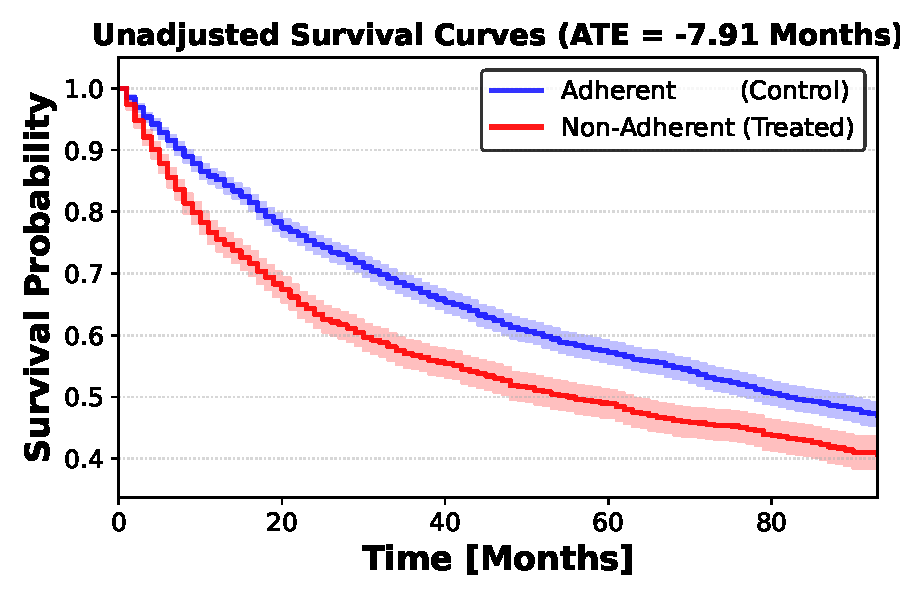
\includegraphics[width=\linewidth]{Appendices/appendix-ch03/images/unadjusted_survival_curves.pdf}
    \caption{Unadjusted Survival Curves obtained from Kaplan-Meier Estimator for \textcolor{blue}{Adherent} (Control) and \textcolor{red}{Non-Adherent} (Treated) Patients. The Average Treatment Effect from the Restricted Mean Event Time difference between the groups is -7.91 Months.}
    \ChThreeFloatLabel{ch03:fig:unadjusted_survival_curve}
\end{figure}



\subsubsection{Complete Ablation Tables}
\label{ch03:apd:ablation}


The complete ablation tables summarize the impact of excluding county-provided risk scores on Average Treatment Effect (ATE) estimates across different models and time snapshots.
Table~\ref{ch03:tab:table_ablation_CoxPH} presents the ATE estimates for the Cox Proportional Hazards (CoxPH) model.
The removal of risk scores results in consistently more negative ATEs across all snapshots, with increases in magnitude most evident at earlier time points, such as 3 months, where the ATE shifts from \(-3.524 \pm 0.274\) to \(-5.432 \pm 0.344\) using the T-learner.
This suggests that risk scores effectively capture confounding factors that partially attenuate the observed impact of non-adherence.

Table~\ref{ch03:tab:table_ablation_RandomSurvivalForest} shows the ablation results for the Random Survival Forest (RSF) model.
Consistent with CoxPH, ablated models produce more negative ATE estimates, highlighting the importance of including risk scores to control for unmeasured confounding.
For instance, at 3 months, the ATE using the T-learner changes from \(-2.317 \pm 0.602\) to \(-5.915 \pm 0.433\), a substantial difference.
This trend persists across later snapshots, though the effect size diminishes as the cohort composition evolves.

DeepSurv ablation results are detailed in Table~\ref{ch03:tab:table_ablation_DeepSurv}.
The standard errors for DeepSurv ATE estimates remain large, both in full and ablated setups, reflecting its limited reliability for causal inference.
Despite this, the removal of risk scores amplifies the negative ATE values, indicating their critical role in adjusting for confounding.
For example, at 6 months, the S-learner's ATE shifts from \(-0.516 \pm 1.284\) to \(-3.130 \pm 1.551\) following ablation.

Table~\ref{ch03:tab:table_ablation_DeepHit} provides the results for DeepHit.
The ATE estimates show high variability, particularly in the ablated models, where standard errors are considerable.
For example, at 9 months, the T-learner ATE for the full model is \(6.887 \pm 5.930\), which reduces to \(2.075 \pm 3.780\) post-ablation.
This variability undermines the interpretability of DeepHit's estimates, underscoring its limitations for both survival and causal analyses in this dataset.

The Causal Survival Forest (CSF) results, presented in Table~\ref{ch03:tab:table_ablation_CausalSurvivalForest}, follow a similar pattern.
The magnitude of ATEs increases following ablation, particularly at earlier snapshots.
At 3 months, the ATE changes from \(-3.045 \pm 0.128\) to \(-7.816 \pm 0.064\), indicating a substantial impact of excluding risk scores.
This trend diminishes at later time points, where selection bias and survivor effects likely play a greater role.

Overall, the ablation results reveal consistent trends across all models.
The exclusion of county-provided risk scores leads to more pronounced negative ATE estimates, highlighting their utility as proxies for unmeasured confounders.
While the observed differences are most pronounced at earlier snapshots, the increasing standard errors at later time points suggest a need for cautious interpretation.
These findings underscore the importance of comprehensive feature inclusion in survival and causal modeling to improve robustness and accuracy.
The trends observed in later time snapshots align with the biases discussed in Appendix~\ref{ch03:apd:causal_inference}, where selection bias and declining survival model performance introduce additional challenges in interpreting ATE estimates.
This further reinforces the difficulty in drawing reliable causal conclusions at these later snapshots, as the subset of patients included becomes increasingly non-representative of the original cohort.


% !TeX root = ../../../main.tex
\begin{table}[hbtp]
    \setlength{\tabcolsep}{4pt}
    \ChThreeFloatContents
      {ch03:tab:table_ablation_CoxPH}
      {\caption{Causal Inference Ablation ATE Estimates for CoxPH}}
      {\adjustbox{max width=.825\textwidth}{\begin{tabular}{l c c c c c }
    \toprule
    &T-learner & S-learner & Matching (1) & Matching (5) & Matching (20) \\
    \midrule
    \textit{(3 months)}
 &  &  &  &  \\
    CoxPH (Full) & -3.524 ± 0.274 & -3.644 ± 0.393 & -4.245 ± 0.005 & -4.280 ± 0.003 & -4.406 ± 0.002 \\
    CoxPH (Ablation) & -5.432 ± 0.344 & -5.460 ± 0.429 & -6.020 ± 0.004 & -6.105 ± 0.004 & -6.184 ± 0.002 \\\\
    \textit{(6 months)}
 &  &  &  &  \\
    CoxPH (Full) & -2.910 ± 0.791 & -2.118 ± 0.751 & -2.578 ± 0.009 & -2.639 ± 0.006 & -2.900 ± 0.007 \\
    CoxPH (Ablation) & -4.933 ± 0.815 & -4.191 ± 0.720 & -4.220 ± 0.007 & -4.287 ± 0.003 & -4.453 ± 0.003 \\\\
    \textit{(9 months)}
 &  &  &  &  \\
    CoxPH (Full) & -2.285 ± 0.578 & -1.384 ± 0.512 & -1.658 ± 0.006 & -1.790 ± 0.002 & -2.032 ± 0.003 \\
    CoxPH (Ablation) & -3.397 ± 0.570 & -2.392 ± 0.495 & -2.148 ± 0.006 & -2.186 ± 0.003 & -2.387 ± 0.002 \\\\
    \bottomrule
    \end{tabular}}}
\end{table}





% !TeX root = ../../../main.tex
\begin{table}[hbtp]
    \setlength{\tabcolsep}{4pt}
    \ChThreeFloatContents
      {ch03:tab:table_ablation_RandomSurvivalForest}
      {\caption{Causal Inference Ablation ATE Estimates for RandomSurvivalForest}}
      {\adjustbox{max width=0.9\textwidth}{\begin{tabular}{l c c c c c }
    \toprule
    &T-learner & S-learner & Matching (1) & Matching (5) & Matching (20) \\
    \midrule
    \textit{(3 months)}
 &  &  &  &  \\
    RandomSurvivalForest (Full) & -2.317 ± 0.602 & -1.183 ± 0.363 & -1.615 ± 0.073 & -1.538 ± 0.054 & -1.978 ± 0.050 \\
    RandomSurvivalForest (Ablation) & -5.915 ± 0.433 & -4.938 ± 0.370 & -5.668 ± 0.078 & -5.647 ± 0.103 & -5.712 ± 0.077 \\\\
    \textit{(6 months)}
 &  &  &  &  \\
    RandomSurvivalForest (Full) & -2.148 ± 0.957 & -0.925 ± 0.378 & -1.762 ± 0.191 & -1.569 ± 0.135 & -1.807 ± 0.109 \\
    RandomSurvivalForest (Ablation) & -5.210 ± 0.898 & -3.805 ± 0.767 & -4.007 ± 0.158 & -3.992 ± 0.163 & -4.307 ± 0.144 \\\\
    \textit{(9 months)}
 &  &  &  &  \\
    RandomSurvivalForest (Full) & -1.468 ± 0.518 & -0.546 ± 0.106 & -1.159 ± 0.042 & -1.242 ± 0.050 & -1.540 ± 0.055 \\
    RandomSurvivalForest (Ablation) & -3.848 ± 0.580 & -2.579 ± 0.394 & -2.554 ± 0.079 & -2.704 ± 0.077 & -2.907 ± 0.076 \\\\
    \textit{(12 months)}
 &  &  &  &  \\
    RandomSurvivalForest (Full) & 0.099 ± 0.430 & 0.050 ± 0.173 & -0.427 ± 0.148 & -0.544 ± 0.134 & -0.829 ± 0.127 \\
    RandomSurvivalForest (Ablation) & -2.238 ± 0.652 & -0.986 ± 0.545 & -1.090 ± 0.022 & -1.343 ± 0.044 & -1.811 ± 0.061 \\\\
    \bottomrule
    \end{tabular}}}
\end{table}




% !TeX root = ../../../main.tex
\begin{table}[hbtp]
    \setlength{\tabcolsep}{4pt}
    \ChThreeFloatContents
      {ch03:tab:table_ablation_DeepSurv}
      {\caption{Causal Inference Ablation ATE Estimates for DeepSurv}}
      {\adjustbox{max width=.825\textwidth}{\begin{tabular}{l c c c c c }
    \toprule
    &T-learner & S-learner & Matching (1) & Matching (5) & Matching (20) \\
    \midrule
    \textit{(3 months)}
 &  &  &  &  \\
    DeepSurv (Full) & -2.366 ± 0.603 & -1.986 ± 0.382 & -2.160 ± 1.014 & -2.101 ± 1.051 & -2.312 ± 1.223 \\
    DeepSurv (Ablation) & -4.775 ± 0.853 & -3.842 ± 2.052 & -4.483 ± 2.070 & -4.529 ± 2.067 & -4.613 ± 2.061 \\\\
    \textit{(6 months)}
 &  &  &  &  \\
    DeepSurv (Full) & -3.685 ± 1.998 & -0.516 ± 1.284 & -1.877 ± 0.708 & -1.927 ± 0.594 & -2.152 ± 0.422 \\
    DeepSurv (Ablation) & -4.406 ± 2.343 & -3.130 ± 1.551 & -2.124 ± 1.442 & -2.129 ± 1.434 & -2.189 ± 1.534 \\\\
    \textit{(9 months)}
 &  &  &  &  \\
    DeepSurv (Full) & -2.144 ± 2.706 & 0.837 ± 0.767 & -0.923 ± 0.446 & -0.928 ± 0.436 & -1.021 ± 0.558 \\
    DeepSurv (Ablation) & -4.979 ± 2.941 & -2.165 ± 2.317 & -2.279 ± 1.823 & -2.366 ± 1.887 & -2.483 ± 2.043 \\\\
    \textit{(12 months)}
 &  &  &  &  \\
    DeepSurv (Full) & -2.650 ± 1.553 & 1.116 ± 0.605 & 0.262 ± 1.353 & -0.025 ± 1.381 & -0.347 ± 1.399 \\
    DeepSurv (Ablation) & -2.267 ± 1.834 & -0.593 ± 1.165 & -0.415 ± 1.082 & -0.700 ± 1.127 & -1.097 ± 1.174 \\\\
    \bottomrule
    \end{tabular}}}
\end{table}




% !TeX root = ../../../main.tex
\begin{table}[hbtp]
    \setlength{\tabcolsep}{4pt}
    \ChThreeFloatContents
      {ch03:tab:table_ablation_DeepHit}
      {\caption{Causal Inference Ablation ATE Estimates for DeepHit}}
      {\adjustbox{max width=.825\textwidth}{\begin{tabular}{l c c c c c }
    \toprule
    &T-learner & S-learner & Matching (1) & Matching (5) & Matching (20) \\
    \midrule
    \textit{(3 months)}
 &  &  &  &  \\
    DeepHit (Full) & -2.956 ± 6.663 & 0.417 ± 0.967 & 0.215 ± 0.481 & 0.241 ± 0.476 & 0.200 ± 0.501 \\
    DeepHit (Ablation) & -5.495 ± 3.492 & -0.936 ± 1.746 & -0.774 ± 0.638 & -0.759 ± 0.622 & -0.806 ± 0.646 \\\\
    \textit{(6 months)}
 &  &  &  &  \\
    DeepHit (Full) & 11.551 ± 3.806 & -1.022 ± 0.428 & 0.007 ± 0.727 & 0.054 ± 0.804 & 0.140 ± 0.876 \\
    DeepHit (Ablation) & -0.249 ± 4.701 & -2.236 ± 1.570 & -1.969 ± 0.660 & -1.915 ± 0.664 & -1.927 ± 0.661 \\\\
    \textit{(9 months)}
 &  &  &  &  \\
    DeepHit (Full) & 6.887 ± 5.930 & 0.169 ± 0.692 & -0.160 ± 0.344 & -0.168 ± 0.328 & -0.163 ± 0.368 \\
    DeepHit (Ablation) & 2.075 ± 3.780 & -1.351 ± 0.895 & -1.273 ± 1.150 & -1.309 ± 1.178 & -1.407 ± 1.222 \\\\
    \textit{(12 months)}
 &  &  &  &  \\
    DeepHit (Full) & 0.822 ± 3.215 & 1.021 ± 0.535 & 0.355 ± 0.424 & 0.256 ± 0.420 & 0.148 ± 0.415 \\
    DeepHit (Ablation) & 6.172 ± 3.723 & 1.118 ± 0.347 & 0.680 ± 0.429 & 0.397 ± 0.315 & 0.078 ± 0.232 \\\\
    \bottomrule
    \end{tabular}}}
\end{table}




% !TeX root = ../../../main.tex
\begin{table}[hbtp]
    \setlength{\tabcolsep}{4pt}
    \footnotesize
    \ChThreeFloatContents
      {ch03:tab:table_ablation_CausalSurvivalForest}
      {\caption{Causal Inference Ablation ATE Estimates for CausalSurvivalForest}}
      {\begin{tabular}{l c }
    \toprule
    &ATE \\
    \midrule
    \textit{(3 months)}
 \\
    CausalSurvivalForest (Full) & -3.045 ± 0.128 \\
    CausalSurvivalForest (Ablation) & -7.816 ± 0.064 \\\\
    \textit{(6 months)}
 \\
    CausalSurvivalForest (Full) & -2.831 ± 0.101 \\
    CausalSurvivalForest (Ablation) & -5.189 ± 0.047 \\\\
    \textit{(9 months)}
 \\
    CausalSurvivalForest (Full) & -1.610 ± 0.057 \\
    CausalSurvivalForest (Ablation) & -2.833 ± 0.077 \\\\
    \textit{(12 months)}
 \\
    CausalSurvivalForest (Full) & 0.345 ± 0.097 \\
    CausalSurvivalForest (Ablation) & -1.561 ± 0.104 \\\\
    \bottomrule
    \end{tabular}}
\end{table}




